\documentclass{article}
\usepackage[utf8]{inputenc}
\usepackage[catalan]{babel}
\usepackage{hyperref}
\usepackage{graphicx}
\usepackage{subfiles}
\usepackage{comment}
\usepackage{titlesec}
\usepackage{hyperref}
% caption and subcaption work together
\usepackage{subcaption} % loads the caption package
\setcounter{secnumdepth}{4}

% Code
\usepackage{listings}
\usepackage{minted}
\usepackage{xcolor}

% Ploting 
\usepackage{pgfplots}
\usepackage{pgfplotstable}
\usepackage{booktabs}
\usepackage{array}
\usepackage{colortbl}

% Ploting settings
\pgfplotstableset{ 
  % global config, for example in the preamble
  every head row/.style={before row=\toprule,after row=\midrule},
  every last row/.style={after row=\bottomrule},
  fixed,precision=2,
}

% Code settings
\definecolor{codegreen}{rgb}{0,0.6,0}
\definecolor{codegray}{rgb}{0.5,0.5,0.5}
\definecolor{codedarkgray}{rgb}{0.75,0.75,0.75}
\definecolor{codepurple}{rgb}{1,0,0}
\definecolor{codedarkpurple}{rgb}{0.65,0,0.8}
\definecolor{codedarkorange}{rgb}{0.85,0.4,0}
\definecolor{backcolour}{rgb}{0.95,0.95,0.95}

\lstdefinestyle{mystyle}{
    frame=tb,
    language=[Sharp]C,
    backgroundcolor=\color{backcolour},   
    commentstyle=\color{codegray},
    keywordstyle=\color{codedarkorange},
    numberstyle=\tiny\color{codegray},
    stringstyle=\color{codegreen},
    basicstyle=\fontsize{9}{10}\selectfont\ttfamily,
    breakatwhitespace=false,         
    breaklines=true,                 
    captionpos=b,                    
    keepspaces=true,                 
    numbers=left,                    
    numbersep=5pt,                  
    showspaces=false,                
    showstringspaces=false,
    showtabs=false,                  
    tabsize=2,
    literate={\ \ }{{\ }}1
}
\lstset{style=mystyle}

\setlength{\parskip}{0.5em}

\titleformat{\paragraph}
{\normalfont\normalsize\bfseries}{\theparagraph}{1em}{}
\titlespacing*{\paragraph}
{0pt}{3.25ex plus 1ex minus .2ex}{1.5ex plus .2ex}

%%------- Definició de l'estructura del titol -------%%
\title{ \textbf{ Aprenentatge per reforç amb Unity} 
\\ {\Large TAIA Project}}
\author{\small Wilber Eduardo Bermeo Quito }
%\date{\small Entrega: 5 de decembre 2021}


% Canvi de nom a la taula de continguts
\renewcommand*\contentsname{Taula de continguts}
\renewcommand\vdots{\vbox{\baselineskip3pt\lineskiplimit0pt\kern1pt\hbox{.}\hbox{.}\hbox{.}\kern-1pt}}

%%------- Inici del documents -------%%
\begin{document}

\maketitle

 % Titol
    \maketitle
    \thispagestyle{empty}
    \newpage
    
    % Taula de continguts
    \tableofcontents
    \newpage
    
    %% ---- start documentation ---- %%
    
    \section{Problema a resoldre en una frase}
    
    Fer que un NPC segueixi una política en concret fent ús de Deep Reinforcement Learning en Unity.

    \section{Introducció i Motivació}
    
    Durant l’estiu del 2021 m’he estat barallant amb Unity (motor de videojocs) perquè vull fer un joc com a treball final de grau.
    
    El joc, resumidament, serà un Metroidvania 2D, en el qual hi haurà una tira de diferents NPCs. Molts d’aquests NPCs seran personatges actius i enemics.

    La motivació és clara, aprendre més d'Unity i expandir la riquesa del TFG amb les eines pròpies d’Unity que dona per implementar intel·ligència artificial als videojocs.  
    
    \section{Dades/Coneixements dels que es disposa}
    
    Degut a la naturalesa del problema seleccionat, no es necessiten conjunts de dades per poder treballar.

    Conec l'entorn de treball Unity, no professionalment, però si tinc un base.
    
    El que em permetrà encarar el problema és l'eina \textit{ML-Agents Toolkit}. Dona totes les eines necessàries per utilitzar Unity com a motor de simulació perquè els Agents de les escenes aprenguin polítiques segons una modelització del problema a resoldre.
    
    \newpage
    
    \section{Proposta}
    
    \subsection{Agent}
    Classe que conté mètodes que poden ser sobre escrits. La seva API contempla mètodes per poder generar observacions del medi, per prendre accions i per assignar recompenses.

    La classe Agent conte altres mètodes que poden ser sobre escrits. Cada Agent està relacionat amb un Behavior Parameter class i a un Decision Requester.
    
    \subsubsection{Com modelitzar un Agent?}
    Es necessiten definir tres tipus d’entitats per cada moment en el joc.
    
    \begin{itemize}
        \item Observacions
        \item Accions
        \item Recompenses
    \end{itemize}
    
    \paragraph{Observacions}
    
    Les observacions poden ser numèriques o visuals. Les observacions numèriques són del punt de vista de l'observador (NPC), les visuals en canvi, són generades per col·lisions de rajos de sensors que es poden ajuntar a l'agent per que tingui informació del terreny i altres objectes en la escena, representen el que l'agent està veient en aquell moment.
    
    \paragraph{Accions}
    
    El que realment l'agent pot fer dintre de l'escena. Les accions poden ser representades per valors continus o discrets.
    
    \paragraph{Recompenses}
   És un escalar que representa que tan bé ho està fent l'agent. Les recompenses (negatives o positives) no tenen per què ser donades a cada moment, es poden donar en certs moments provocats per esdeveniments. És important saber quan i quant es recompensa o es castiga a l'agent pel seu acte. Depenent de la política de recompenses farà que l'aprenentatge d'una certa tasca sigui més ràpida o més lenta.
    
    \subsection{Polítiques a aprendre}
   Els següents dos punts són els problemes a modelitzar perquè l'Agent aprengui la política adequada per compliar-los.
    
    \subsubsection{Autonomia en el moviment}
    
    (v1)

    L'NPC ha de ser capaç de moure d'esquerra a dreta de manera cíclica.
    
    Arribar al màxim rang de desplaçament tant d'esquerra a la dreta ha de donar feedback positiu, però no ha de passar que es quedi en un extrem sense moure, només s'ha de poder atorgar feedback positiu i s'ha vingut de l'altre extrem, un cas excepcional seria la primera vegada que apareix en l'entorn del joc, ja que surt del centre del desplaçament.
    
    En cas de col·lisions amb objectes que no siguin targets d'atac dintre del seu rang ha de poder ser capaç de girar i fer el recorregut contrari. (no es fa). \\
    
    (v2.1, v2.2, v2.3)
    
    L'Agent a més a més de desplaçar-se d'esquerra a dreta ara té l'habilitat de poder fer salts. Els salts únicament estan pensats per canviar a mode d'atac.
    En cas de fer un salt innecessari, l'Agent és veurà castigat. D'aquest amanerà mantindrà el moviment cíclic de la primera versió, però tindrà la capacitat de saltar.
    Que es considera com a salt innecessari?, doncs saltar quan no està sobre el terra o quan no hi hagi enemics detectats.
    
    \subsubsection{Saber atacar}
    
    (v2.1, v2.2, v2.3)
    
    Un cop l'Agent hi hagi après a moure's, la meva idea és que l'NPC detecti entitats a atacar.
    
    Aquestes entitats únicament seran detectades pels rajos del sensor que el NPC té incorporat. L'objectiu en aquest cas és que, deixi de fer el moviment cíclic d'esquerra a dreta i que salti sobre l'objectiu fent col·lisió, les col·lisions encertades donaran feedback positiu.
    
    L'agent mor si és tocat per l'enemic quan aquest no està en mode atac que és el mateix a dir, no haver fet el salt moments abans de la col·lisió amb l'enemic.


    \newpage
    
    \subsection{Arquitectura, Algorismes, Propostes existents}
    
    L'arquitectura del problema que abordo bé donat per les eines que utilitzo per resoldre-ho, en aquest cas \textit{ML-Agents Toolkit}. A part de les eines de \textit{ML-Agents Toolkit} faré servir \textit{Tensorboard} per veure les estadístiques d'aprenentatge.

    A continuació explicaré com és l'arquitectura de ML-Agents Toolkit. ML-Agents Toolkit té els següents quatre blocs com a estructura principal.
    
    \begin{itemize}
        \item Espai d'aprenentatge (Escena d'Unity)
        \item Comuniador (Broquer que connecta Unity amb l'API de Python)
        \item Python API
        \item Python Trainers
    \end{itemize}

    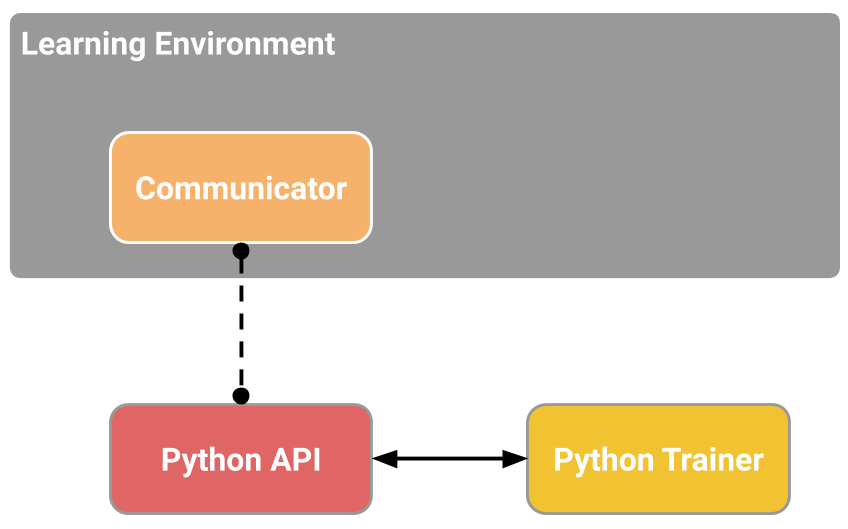
\includegraphics[width=\textwidth]{images/learning_environment_basic.png}
    
    \newpage
    
    \subsubsection{Espai d'aprenentatge}
    Aquí està l'escena d'Unity i els personatges. Els personatges que per requeriment del problema s'han definit com a Agents, podran observar, prendre decisions i tenir recompenses.
    
    \subsubsection{Agent}
    Aquí està l'escena d'Unity i els personatges. Els personatges que per requeriment del problema s'han definit com a Agents, podran observar, prendre decisions i tenir recompenses.
    \begin{itemize}
        \item Initialize
        \item OnEpisodiBegin
        \item OnActionReceived
        \item CollectObservations
        \item Heuristic
    \end{itemize}
    
    \newpage
    
    \paragraph{Initialize}
    Aquest mètode es crida un cop únicament en el cicle de vida de l'aprenentatge. Està pensat per fer caching d'objectes de l'escena o inicialitzar valors.
    
    \paragraph{OnEpisodiBegin}
    Aquest mètode es crida cada cop que un episodi d'aprenentatge ha acabat, forçadament o perquè el màxim nombre de passos de l'episodi s'han completat.
    
    \paragraph{OnActionReceived}
    Aquest mètode porta un paràmetre d'entrada, anomenat ActionBuffer, l'ActionBuffer, és un objecte que té dos arrays, un per poder representar valors continus i altres per representar valors discrets.
    
    Aquest mètode interactua tant amb el mètode \textit{heuristic} i amb el motor d'aprenentatge automàtic.
    
    \paragraph{CollectObservations}
    Aquest mètode s'executa cada x temps, aquest temps d'execució es configura amb l'eina d'Unity.
    
    El mètode té com a paràmetre una estructura de dades semblants com a paràmetre d'entrada que el mètode OnActionReceived. En aquest cas no està pensat per consumir les dades sinó per modificar aquesta referència i per donar informació al motor de Reinforcement Learning quan estem en mode de \textit{Learning}.


    \paragraph{Heuristic}
    Aquest mètode permet interactuar amb el jugador. Fixat que té la mateixa estructura de dades com a paràmetre que el mètode ActionBuffers.
    
    Els valors que s'emplenin en els buffers d'aquesta estructura de dades aniran a parar al mètode \textit{OnActionReceived}.
    
    \newpage
    
    \subsubsection{Behaviour}
    Script que esta pensat per parametritzar i relacionar l’Agent amb la configuració externa a Unity.
    
    Un Behavior pot tenir els següents comportaments:
    \begin{itemize}
        \item Learning
        \item Heuristic
        \item Inference
    \end{itemize}
    
  \paragraph{Learning}
    Quan el \textit{Behavior} està en mode \textit{Learning} vol dir que utilitza el model generat per la sobreescriptura dels mètodes de la clase \textit{Agent} per aprendre. En aquest mode Unity es connecta amb el procés de \textit{mlagents-learn} per generar la xarxa neuronal que representa l'aprenentatge del model.
    
    \paragraph{Heuristic}
    En aquest mode no hi ha procés d'aprenentatge, es fa servir la funció \textit{heuristic} de la classe \textit{Agent} per interactuar amb l'Agent.
    
   \paragraph{Inference}
    Quan el \textit{Behavior} està en mode \textit{Inference} implica que hi ha una xarxa neuronal amb una política apresa, i l'objecte que té aquesta xarxa neuronal es comportarà segons el que s'hi hagi après.
    
    \newpage
    
    \subsubsection{Requester}
    És un Script que serveix per forçar que l'Agent prengui decisions, sense aquest Script com a Component en el nostre Agent, l'Agent mai prendrà decisions. Aquí es pot configurar el període de decisions.
    
    En la següent imatge hi ha les tres diferents arquitectures que podem tenir segons quin comportament tingui el component \textit{Behavior} del objecte Agent. \\
    
    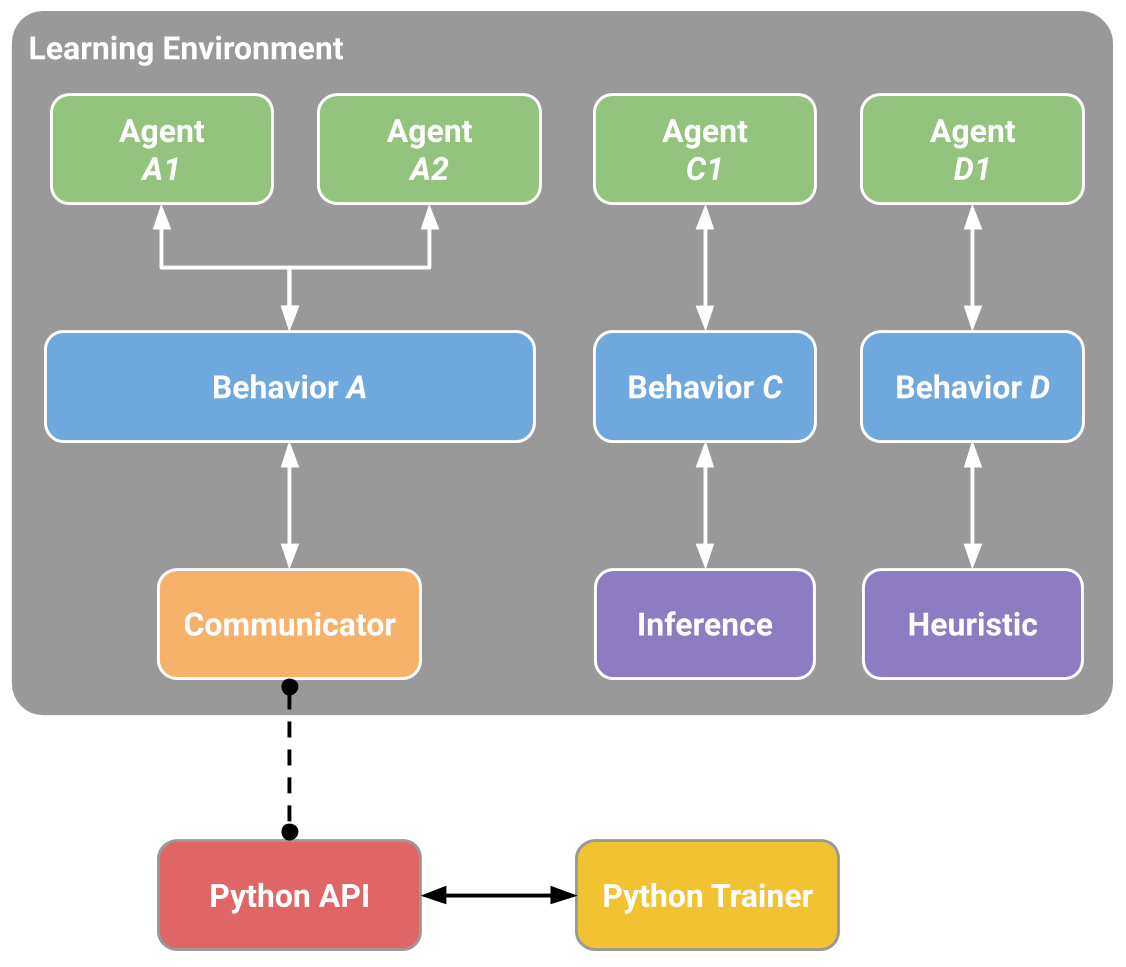
\includegraphics[width=\textwidth]{images/arquitecture_mlagent.png}
    
    \newpage
    
    \subsubsection{Tensorboard}
    Quan l'entrenament s'està executant, ML-Agents Toolkit guarda estadístiques dintre del directori resolts en un directori amb nom únic, donat a l'hora d'executar el procés mlagents-learn.

    Per observar el procés d'entrenament quan està corrent el procés o quan no, ens apropem a la carpeta de resultats i executem: tensorboard –logdir */results\$\{training id\}.
    
    Això obrirà un servidor per servir el contingut estàtic en un dels ports de la teva màquina.
    
    Explicaré alguna de les gràfiques que \textit{Tensorboard} genera, ja que molt segurament les veurem més endavant en cada un de les versions de l'Agent.
    
    \paragraph{Cumulative Reward}
    Gràfica que representa la mitja de el que guanya l'Agent per episodi. Un bon procés d'aprenentatge gènera una gràfica ascendent que en algun moment s'estanca, ja que la seva mitja per episodi és manté.
    
    \paragraph{Learning Rate}
      Representa el temps que li pren per pas a l'algoritme d'entrenament per trobar la política òptima. Hi ha de decréixer linealment en cas que l'aprenentatge s'estigui fent correctament.
        
    \paragraph{Episodi Length}
    Representa la durada mitjana per episodi. Aquesta gràfica depèn de la implementació del model, ja que segons la característica del problema es pot forçar el reinici d'episodi, o potser el problema és maximitzar o minimitzar el temps de vida de l'Agent.
    
    \paragraph{Policy Loss}
    Representa quan la política de l'Agent canvia, un model correcte tendirà a fer una gràfica descendent.
    
        
    \paragraph{Value Loss}
    Representa que tan bé el model es capaç de predir el valor de cada estat. La gràfica ha d'incrementar mentre l'Agent aprèn, però quan la mitja de premi s'estableix ha de descendir
    
    \paragraph{Entropy}
    Representa que tan aleatoris són els moviments de l'Agent, un model correcte expressa una gràfica d'Entropia descendent, ja que significa que realment està aprenent una política i no està fent tants d'intents per provar coses noves.
    
    \textbf{Arquitectura final}
    
    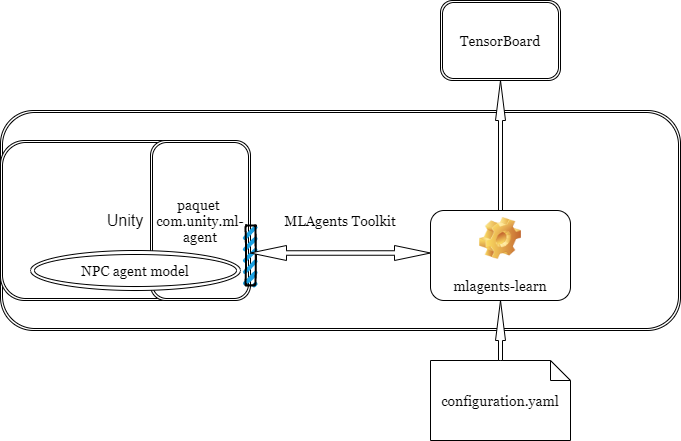
\includegraphics[width=\textwidth]{images/arquitectura-tools.drawio.png} 
    
    \newpage
    
    \section{Experiments}
    
    Aquest projecte conté un seguit d'experiments basats en fases.
    Les fases venen donades per l'apartat \textit{4.2 Polítiques a aprendre}.
    
    \subsection{ Representació de l'objecte NPC dintre d'Unity }
    L'objecte NPC està format tres objectes fills.
    
    \subsubsection{Versió 1}
    
    \begin{itemize}
        \item Limit esquerra
        \item Limit dret
        \item Agent
        \begin{itemize}
            \item Raig esquerra
            \item Raig dret
            \item Body
        \end{itemize}
    \end{itemize}

    Els objectes de límits, són objectes buits i invisibles que tenen un comportament de trigger de esdeveniments en cas de col·lisions. Aquests objectes són essencials per poder delimitar el rang de moviment de l'Agent.

    L'objecte Agent conte el Script de modelatge que hereta de la classe \textit{Agent} a més dels Scripts \textit{Behavior Parameters} i \textit{DesitionRequester}.
    
    Finalment tenim els rajos, que interaccionen amb elements de l'escena. El funcionament d'aquests rajos s'explica en l'apartat \textit{4.1.1.1 Observacions}. \\
    
    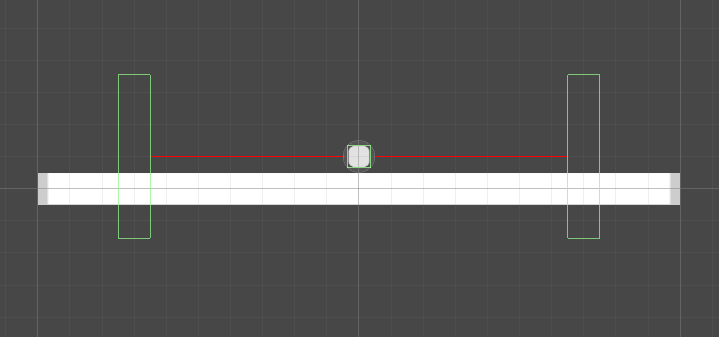
\includegraphics[width=\textwidth]{images/NPC_scene.png} 
    
    \subsubsection{Versións 2.1, 2.2, 2.3}
    L'arquitectura en Unity del NPC és manté, però canvien la quantitat de rajos de raytraicing llençats pels dos sensors. Noteu en la següent imatge que:
    \begin{itemize}
    \item Els rajos frontals són més llargs que els posteriors, d'aquesta manera es dona més realisme al fet que es veu més cap endavant que no a les espatlles
    \item Els rajos estan dispersats en forma de ventall per cobrir més terreny i saber si algu a entrat a la zona d'atac.
    \end{itemize}

    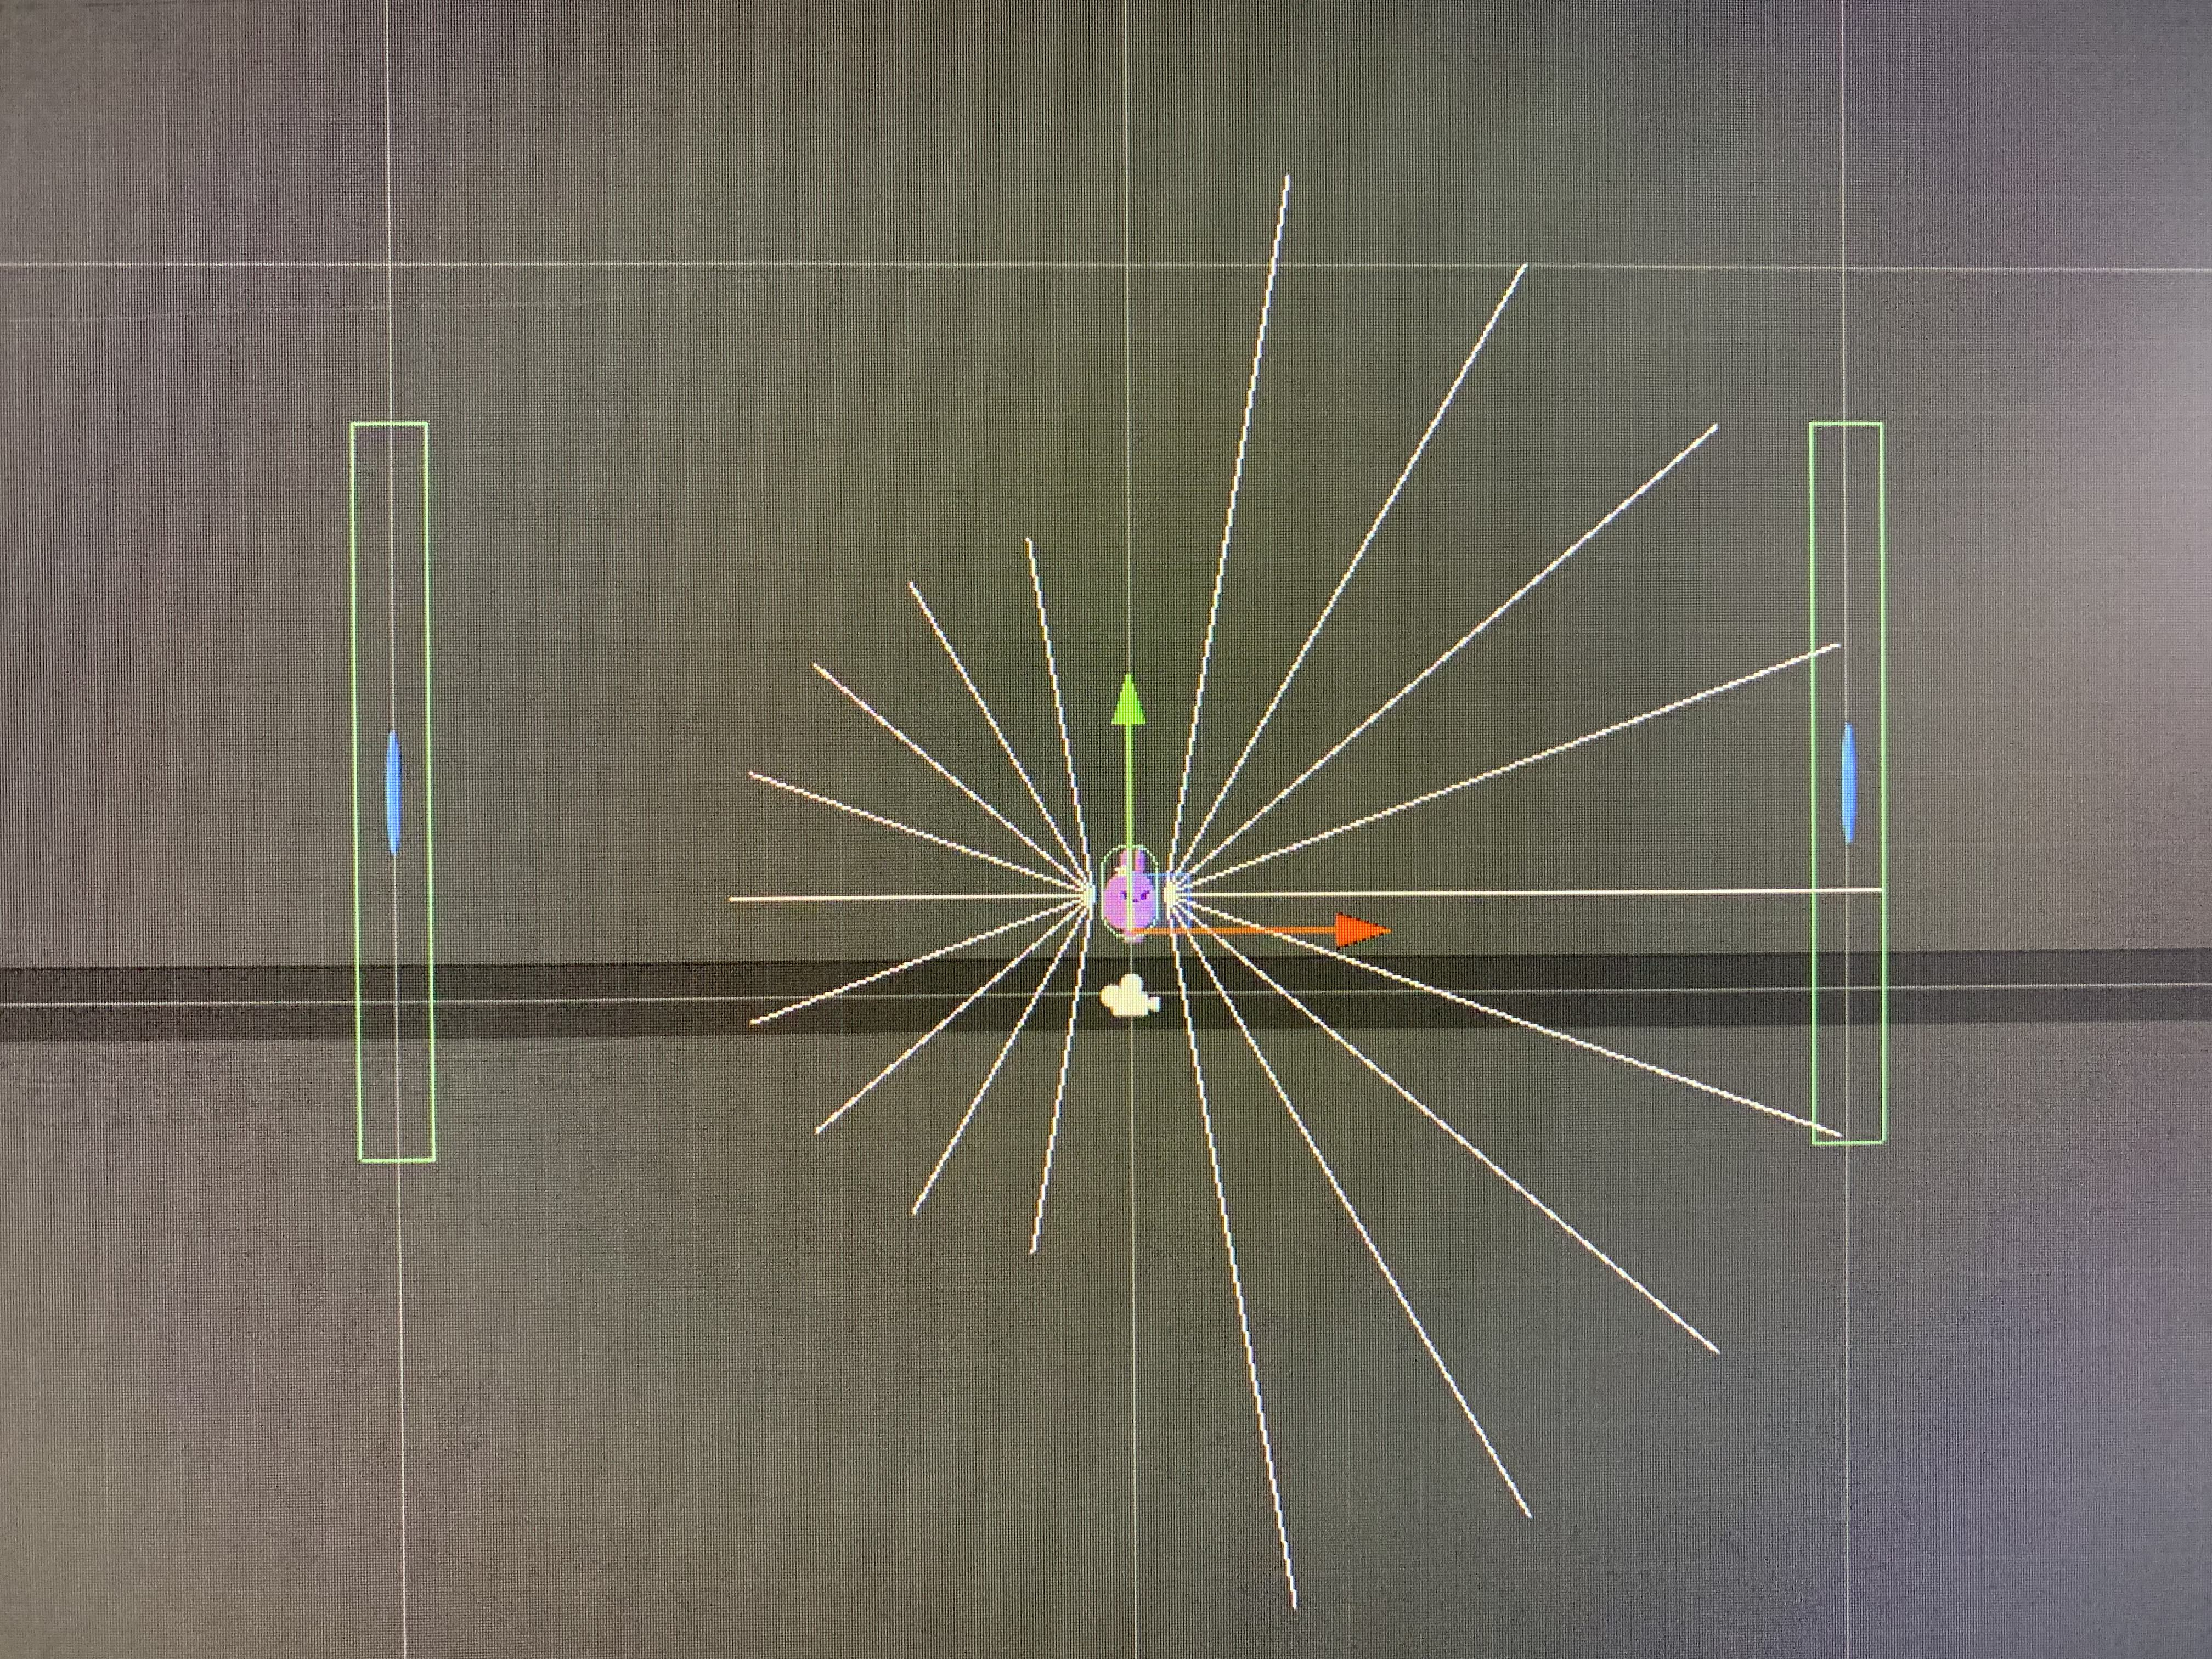
\includegraphics[width=1\textwidth]{images/v2/arq-v2.jpg}

   
   \newpage
    
    \subsection{Metodologia i Resultats}
    
    \subsubsection{Versió 1}
    
    
     Els mètodes que s'hi han sobreescrit de la classe \textit{Agent} són els següents:
    
    \begin{itemize}
        \item Initialize
        \item OnEpisodiBegin
        \item OnActionReceived
        \item CollectObservations
        \item Heuristic
    \end{itemize}
    
    Altres mètodes de classe no propis de la classe \textit{Agent} i que són interessants per poder explicar la modelització del problema:
    
    \begin{itemize}
        \item OnTriggerEnter2D
        \item OnTriggerExit2D
    \end{itemize}
    
    \paragraph{Initialize}
    
   Rutina que s'executa només un cop quan es dona play al motor d'Unity.

    Agafo el component de l'objecte que em permet treballar amb les físiques de Unity. El component és el \textit{RigidBody} que ha d'haver estat afegit a l'objecte com una component des de l'interficie d'Unity. El component \textit{RigidBody} ha de tenir el comportament de \textit{Dynamic} perquè sigui afectat per la gravetat de configurada en l'escena.
    
    Per altra banda configuro el nombre de passos per episodi a zero, en cas que l'estat de la variable \textit{trainingMode} sigui fals. Aquesta configuració em permet fer proves en mode \textit{Heuristic} o en mode \textit{Inferencia} sense passar pel cicle de vida \textit{OnEpisidoBegin}.
    
    La variable \textit{MaxStep} és una variable pròpia de la classe \textit{Agent} i representa el nombre de passos màxims que es fan durant l'Agent està aprenent una política. Quan s'ha fet aquests nombres de passos, immediatament pel cicle de vida de l'Agent, força l'execució de la rutina \textit{OnEpisodiBegin}. \\
    
    \begin{lstlisting}
    public override void Initialize()
    {
        _rigidbody2D = GetComponent<Rigidbody2D>();
        // infinite steps for session
        if (!trainningMode) MaxStep = 0;
    }
    \end{lstlisting}
    
    
    \newpage
    
    \paragraph{OnEpisodeBegin}
    
    El següent mètode s'executa a l'inici de cada episodi. És important de restablir els estats inicials d'algunes propietats de l'Agent, degut a què l'Agent manté la inèrcia del episodi anterior.

    En la rutina es treu l'inèrcia que tenia l'Agent en l'episodi anterior, se'l reposiciona al centre i s'escull una meta aleatòriament. A aquestes altures les metes a escollir són els límits.
    
    \begin{lstlisting}
    public override void OnEpisodeBegin()
    {
        // reseting movement inercy
        _rigidbody2D.velocity = Vector2.zero;
        //reseting positions
        transform.position = transform.parent.position;
        // changin randomnes
        Random.InitState(System.DateTime.Now.Millisecond);
        // finding the moving target
        FindMovingTarget();
    }
    \end{lstlisting}
    
    \paragraph{OnActionReceived}
    
    La lògica dintre d'aquests mètode determina el comportament de l'Agent.
    Les accions que s'esperen és una continua, un valor entre menys u i més u. Segons aquesta acció la velocitat de l'Agent serà donada.
    
    \begin{lstlisting}
    // called when action is received from either {player, neural network}
    // each buffer position refers to an action, I decide what it means for each positions
    // inside that structure has continuous and discrete actions
    // index 0: -1 means move to the left, +1 means move to the right
    // the cool thing about the neural network, is that it figures it all automatic
    public override void OnActionReceived(ActionBuffers actions)
    {
        Vector2 movement = new Vector2(actions.ContinuousActions[0] * movementForce, 0);
        _rigidbody2D.velocity = movement;
    }
    \end{lstlisting}
    
    \paragraph{CollectObservations}
    
    En aquest mètode li he de donar al procés d'aprenentatge aquells paràmetres que jo crec que són importants per tenir en compte a l'hora d'aprendre la política.

    Aquí vaig trobar interessant d'informar el procés d'aprenentatge, quina és la horientació del Agent respecte el punt objectiu. La distància de l'Agent respecte el punt objectiu, la posició del punt objectiu i finalment la velocitat de moviment de l'Agent.
    
    \begin{lstlisting}
    // Should include all variables relevant for following 
    // to take the agent the optimally informed desition.
    // No extraneous information here please
    public override void CollectObservations(VectorSensor sensor)
    {
        if (!currentTarget) return;

        Vector2 currentPos = new Vector2(transform.position.x, 0);
        Vector2 targetPos = new Vector2(currentTarget.position.x, 0);

        Vector2 toTarget = targetPos - currentPos;
        // 2 observations (horientation)
        sensor.AddObservation(toTarget.normalized);
        // 1 observation (distance)
        sensor.AddObservation(Vector2.Distance(targetPos, currentPos));
        // 2 observations for current target position
        sensor.AddObservation(targetPos);
        // 2 observations for movement velocity
        sensor.AddObservation(_rigidbody2D.velocity);
        // Note: curiosamente si normalizo la velocidad, le cuesta mucho aprenderx
    }
    \end{lstlisting}
    
    
    
    
    
   
   \newpage
   
   \paragraph{Heuristic}
   
   En aquesta versió únicament l'Agent ha de poder interpretar valors entrats per teclat que representin moviments laterals.
    
    Es modifica la referència dels \textit{ActionBuffers} de tal manera que en el buffer de variables contínues és passa el valor entrat per teclat. \\
   
   \begin{lstlisting}
   // this method allows me to interact with the game
    // when the ml agents is not set to trainning
    public override void Heuristic(in ActionBuffers actionsOut)
    {
        ActionSegment<float> continuosActions = actionsOut.ContinuousActions;
        var force = Input.GetAxis("Horizontal");
        continuosActions[0] = force;
    }
   \end{lstlisting}
   
    
    L'objectiu de fer aprendre la política de moure's cíclicament ha sigut tot un èxit.
    
    Perquè el temps d'aprenentatge es fes més curt, el que vaig fer va ser duplicar l'Agent quatre vegades. \\
        
    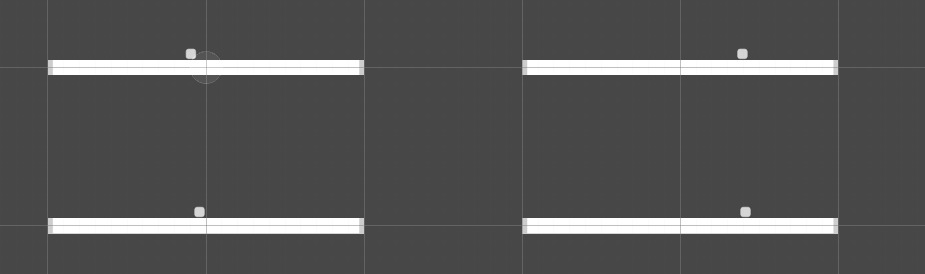
\includegraphics[width=\textwidth]{images/v1/autonomia_v1.jpeg}
    
    Fixem-nos en els següents logs que \textit{mlagents-learn} va soltant en el procés d'aprenentatge. \\
    
    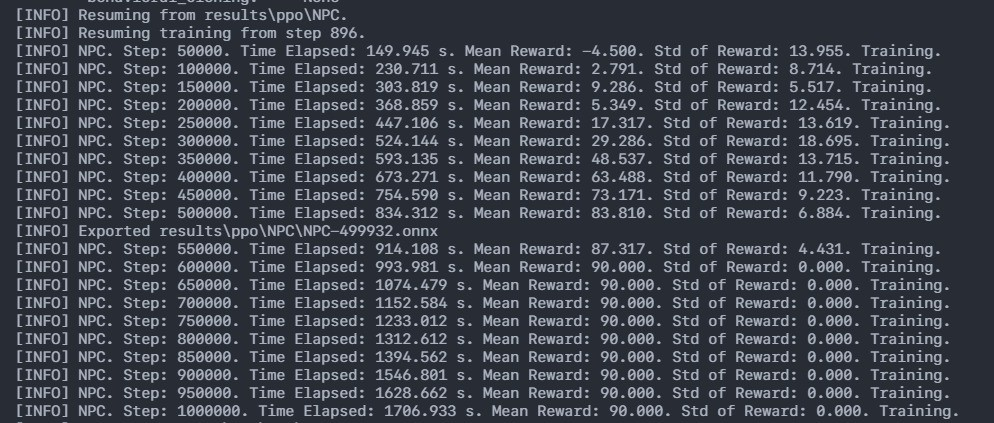
\includegraphics[width=\textwidth]{images/v1/log_v1.jpeg}
    
    Cada una de les entrades del log representen episodis. Les primeres entrades donen una mitja \textit{Mean Reward} que les últimes i la desviació estàndard és bastant més ample que les últimes.
    
    Finalment arriba el moment on l'aprenentatge de l'Agent no canvia. Això vol dir que ha après una política i immediatament, \textit{mlagents-learn} quan veu que la mitja per cada episodi és la mateixa tanca el procés d'aprenentatge.
    

    A continuació veurem algunes gràfiques que \textit{Tensorboard} ens ha generat respecte a aquest procés d'aprenentatge.
    
    \begin{figure}[H]
        \begin{figure}[H]
        \centering
            \subcaptionbox{Comulative reward}{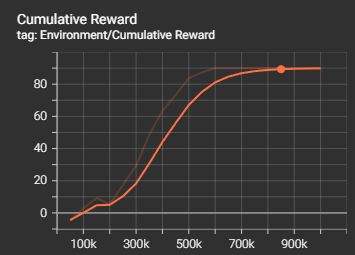
\includegraphics[width=0.30\textwidth]{images/v1/comulative_reward_autonomia_v1.png}}%
            \hfill % <-- Seperation
            \subcaptionbox{Episodi length}{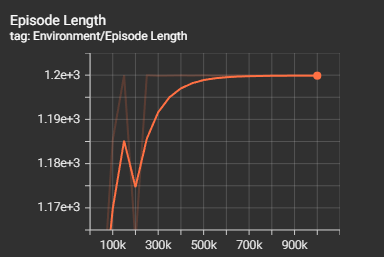
\includegraphics[width=0.30\textwidth]{images/v1/episode_length_autonomia_v1.png}}%
            \hfill % <-- Seperation
            \subcaptionbox{Learning rate}{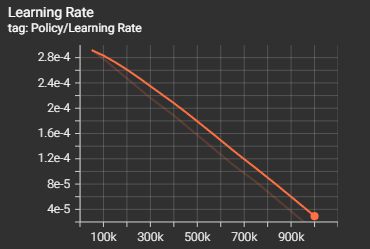
\includegraphics[width=0.30\textwidth]{images/v1/learning_rate_v1.png}}%
            \hfill % <-- Seperation
             \subcaptionbox{Policity loss}{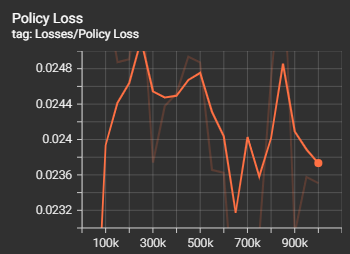
\includegraphics[width=0.30\textwidth]{images/v1/policity_loss_autonomia_v1.png}}%
            \hfill % <-- Seperation
            \subcaptionbox{Value Loss}{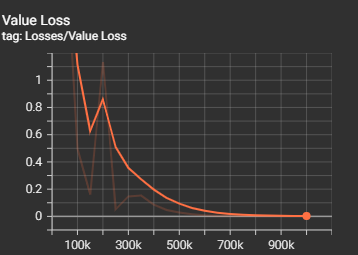
\includegraphics[width=0.30\textwidth]{images/v1/value_loss_autonomia_v1.png}}%
            \hfill % <-- Seperation
            \subcaptionbox{Entropy}{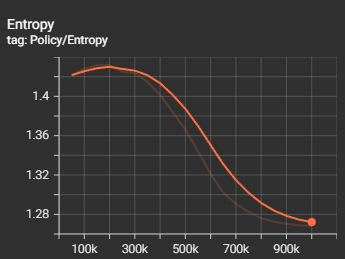
\includegraphics[width=0.30\textwidth]{images/v1/entropy_autonomia_v1.png}}%
            
        \end{figure}
    \end{figure}
    
    \newpage
    
    \subsubsection{Versió 2.1}
    
       La versió 1 i la versió 2.1 i superiors no són compatibles perquè s'ha incrementat el nombre de rajos per sensor de detecció, i Unity es queixa i no deixa reutilitzar la xarxa neuronal de la versió 1.

    L'Agent en la versió 2.1 és capaç de fer salts i ja va estar preparat per poder atacar a possibles enemics (encara que aquestes funcionalitat no està polida). A la versió 2.1 no se li incorpora interactivitat amb enemics, es fan les proves per veure si amb els canvis que s'han fet respecta versió 1, el NPC segueix sent capaç de fer el desplaçament cíclic.
    
    Els canvis que s'han fet en la versió 2.1 fan que el NPC tingui una interacció de tipus continua (0,1) que representa el fet de saltar.
    Si s'activa l'objecte HeroGenerator de l'escena podem veure que l'Agent tindrà dificultats, ja que els objectes generats col·lisionaran amb ell.
    
    Aquesta versió sobreescriu els mateixos mètodes de la classe Agent, però amb refactoritzacions i ampliació de lògica en alguna d'elles.
    
    Métodes sobrescrits que és mantén igual:
    \begin{itemize}
    \item Collect observations
    \item Initialize
    \end{itemize}
    
    \paragraph{OnEpisodeBegin}
    En aquesta versió es pot veure quan l'Agent a col·lisionat amb un dels límits, cada cop que s'inicialitza un entrenament, aquest els torna al seu estat inicial. Per la resta és pràcticament igual excepte per la crida a la funció PickOneLimitAsTarget que abans es deia FindMovingTarget.
    
    \begin{lstlisting}
     public override void OnEpisodeBegin()
    {
        // reseting movement inercy
        rb.velocity = Vector2.zero;
        //reseting positions
        transform.position = transform.parent.position;
        // changin randomnes
        Random.InitState(System.DateTime.Now.Millisecond);
        // current target rebooted
        target = null;
        // setting attack mode to false`
        attackMode = false;
        // finding the moving target
        PickOneLimitAsTarget();
        // restart limits
        RestartLimits();
    }
    \end{lstlisting}
    
    \newpage
    
    \paragraph{OnActionReceived}
    Aquest és un dels mètodes que ha canviat més. Obliga al fet que l'Agent faci la tasca el ràpid possible, castiga a l'Agent en cas de fer salts innecessaris i premia en cas que l'orientació donada per l'aprenentatge estigui orientada cap al target.
    
    \begin{lstlisting}
   // called when action is received from either {player, neural network}
    // each buffer position refers to an action, I decide what it means for each positions
    // inside that structure has continuos and discrete actions
    // index 0: -1 means move to the left, +1 means move to the right
    // the cool thing about the neural network, is that it figurates it all automatic

    // the second element is discrete parameter, which says jump or not [0,1]
    // when npc jumps has the hability to make damage and only should jump when there is a enemy nearby
    // and it is in the ground.

    // in case it is not in the ground and there is no enemy nearby I penalize the agent

    // as I want to make the agent move to target as quick as possible, each time
    // on action received is executed I penalize him

    // in case the action given to move target is well oriented I give him a little reward
    public override void OnActionReceived(ActionBuffers actions)
    {
        int jump = actions.DiscreteActions[0];
        float xhorientation = actions.ContinuousActions[0];
        Vector2 v = rb.velocity;

        AddReward(-gain / 10000); // trying to finish the task quickly 

        // checking if the new orientantion action is good
        if (target)
        {
            Vector2 orientation = new Vector2(xhorientation, 0).normalized;
            float simil = Vector2.Dot(orientation, TargetDirectionNormalized());

            if (simil > Mathf.Epsilon)
            {
                Debug.Log("Well oriented");
                Debug.Log(simil);
                AddReward(gain / 100);
            }

        }
        // try to learn not to jump when it is not in the ground
        bool unneededJump = jump == 1 && !ShouldJump();
        if (unneededJump)
        {
            Debug.Log("Unneded jump");
        }
        if (trainning && unneededJump)
        {
            AddReward(-gain);
            EndEpisode();
        }

        // run attack mode
        if (jump == 1 && !attackMode)
        {
            StartCoroutine(AttackModeCoroutine());
        }

        Vector2 movement = new Vector2(xhorientation * movementPower, jump == 1 ? jump * jumpPower : v.y);
        rb.velocity = movement;
    }

    \end{lstlisting}
    
    \paragraph{Heuristic}
    El canvi en aquest mètode hi ha sigut mínim, el canvi principal és permetre al jugador fer un salt amb la tecla Scape si l'Agent està situat a terra.
    
    \begin{lstlisting}
      
     // this method allows me to interact with the game
    // when the ml agents is not set to trainning
    public override void Heuristic(in ActionBuffers actionsOut)
    {
        ActionSegment<float> continuosActions = actionsOut.ContinuousActions;
        ActionSegment<int> discreteActions = actionsOut.DiscreteActions;

        discreteActions[0] = Input.GetKey(KeyCode.Space) && IsGrounded() ? 1 : 0;
        continuosActions[0] = Input.GetAxis("Horizontal");
    }
    
    \end{lstlisting}
  
    Estadístiques llençades per Tensorboard de l'entrenament de la versió 2.1.
    
    \begin{figure}[H]
        \begin{figure}[H]
        \centering
            \subcaptionbox{Comulative reward}{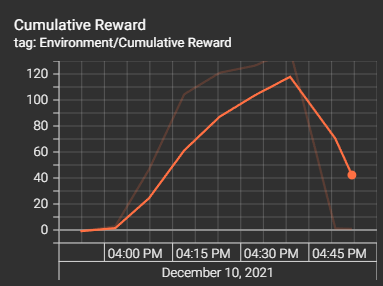
\includegraphics[width=0.30\textwidth]{images/v2/1/cumulativereward.png}}%
            \hfill % <-- Seperation
            \subcaptionbox{Episodi length}{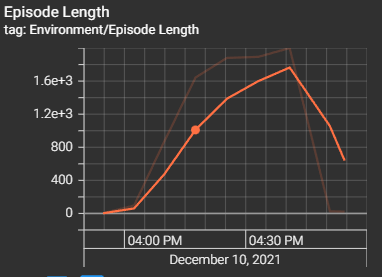
\includegraphics[width=0.30\textwidth]{images/v2/1/episodilength.png}}%
            \hfill % <-- Seperation
            \subcaptionbox{Learning rate}{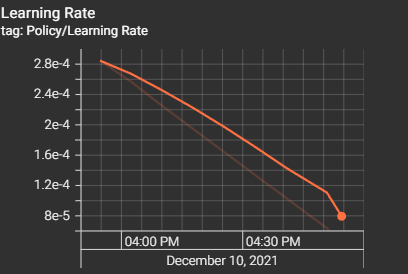
\includegraphics[width=0.30\textwidth]{images/v2/1/learningrate.png}}%
            \hfill % <-- Seperation
             \subcaptionbox{Policity loss}{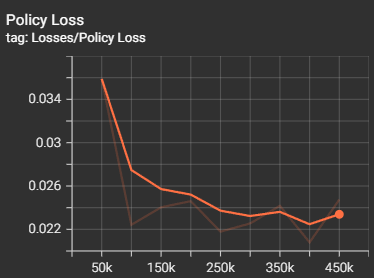
\includegraphics[width=0.30\textwidth]{images/v2/1/policityloss.png}}%
            \hfill % <-- Seperation
            \subcaptionbox{Value Loss}{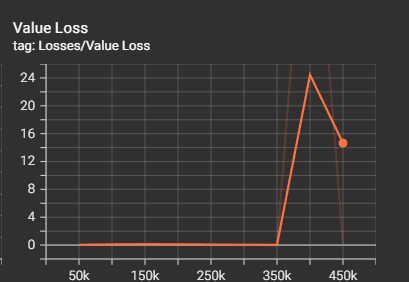
\includegraphics[width=0.30\textwidth]{images/v2/1/valueloss.png}}%
            \hfill % <-- Seperation
            \subcaptionbox{Entropy}{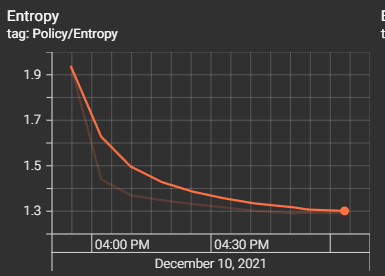
\includegraphics[width=0.30\textwidth]{images/v2/1/entropy.png}}%
        \end{figure}
    \end{figure}
    
    \newpage
    
     \subsubsection{Versió 2.2}
    La versió 2.2 és l'ampliació de la versió 2.1, en aquest cas els processos d'entrenament tindran en compte el factor enemic i es fa que aprengui a no col·lisionar amb ells sense estar en mode atac. Té alguns falles que es milloren en la versió v2.3.

    El canvi més significatiu es fa en el mètode OnActionReceived, en la versió 2.1 a l'Agent se'l castigava per saltar quan no havia de fer-ho i s'acabava i es forçava l'acabament de l'episodi d'aprenentatge, en aquesta versió se'l castiga però de forma més lleu i no  s'acava el procés d'aprenentatge, a més a més de donar-li un petit incentiu quan ha fet un salt correcte.
     
     \begin{lstlisting}
       public override void OnEpisodeBegin()
    {
        Debug.Log("New episode...");
        // reseting movement inercy
        rb.velocity = Vector2.zero;
        //reseting positions
        transform.position = transform.parent.position;
        // changin randomnes
        Random.InitState(System.DateTime.Now.Millisecond);
        // current target rebooted
        // setting attack mode to false`
        // removes enemis from scene
        if (heroGenerator)
        {
            heroGenerator.Clean();
        }
        attackMode = false;
        target = null;
        // finding the moving target
        PickOneLimitAsTarget();
        // restart limits
        RestartLimits();
    }
    \end{lstlisting}
    
       \begin{lstlisting}
      // in case it is not in the ground and there is no enemy nearby I penalize the agent
    // as I want to make the agent move to target as quick as possible, each time
    // on action received is executed I penalize him
    // in case the action given to move target is well oriented I give him a little reward
    public override void OnActionReceived(ActionBuffers actions)
    {
        int jump = actions.DiscreteActions[0];
        float xhorientation = actions.ContinuousActions[0];
        Vector2 v = rb.velocity;
        AddReward(-gain / 10000); // trying to finish the task quickly 
        // checking if the new orientantion action is good
        if (target)
        {
            Vector2 orientation = new Vector2(xhorientation, 0).normalized;
            float simil = Vector2.Dot(orientation, TargetDirectionNormalized());

            if (simil > Mathf.Epsilon)
            {
                AddReward(gain / 100);
            }

        }
        bool shouldJump = ShouldJump(); // SHOULD JUMP WHEN NOT IN MODE ATTACK TOO
        // try to learn not to jump when it is not in the ground
        bool unneededJump = jump == 1 && !shouldJump;

        bool goodJump = jump == 1 && shouldJump;

        if (trainning && unneededJump)
        {
            Debug.Log("Unneded jump...");
            AddReward(-gain / 100);
            // EndEpisode(); // CLAVE!!!
        }

        if (trainning && goodJump) // CLAVE
        {
            Debug.Log("Good jump...");
            AddReward(gain / 10);
        }
        Vector2 movement = new Vector2(xhorientation * movementPower, jump == 1 && shouldJump ? jump * jumpPower : v.y); // CLAVE
        rb.velocity = movement;
        // run attack mode
        if (jump == 1 && !attackMode)
        {
            StartCoroutine(AttackModeCoroutine());
        }
    }
    \end{lstlisting}

    Estadístiques llençades per Tensorboard de l'entrenament de la versió 2.2. 
    
    \begin{figure}[H]
        \begin{figure}[H]
        \centering
            \subcaptionbox{Comulative reward}{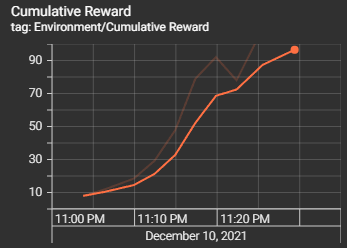
\includegraphics[width=0.30\textwidth]{images/v2/2/cumulativereward.png}}%
            \hfill % <-- Seperation
            \subcaptionbox{Episodi length}{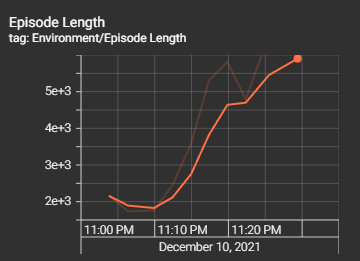
\includegraphics[width=0.30\textwidth]{images/v2/2/episodilength.png}}%
            \hfill % <-- Seperation
            \subcaptionbox{Learning rate}{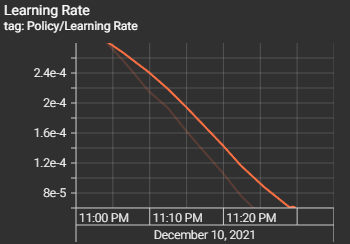
\includegraphics[width=0.30\textwidth]{images/v2/2/learningrate.png}}%
            \hfill % <-- Seperation
             \subcaptionbox{Policity loss}{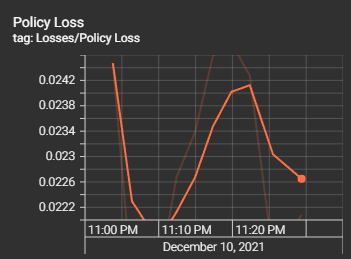
\includegraphics[width=0.30\textwidth]{images/v2/2/policyloss.png}}%
            \hfill % <-- Seperation
            \subcaptionbox{Value Loss}{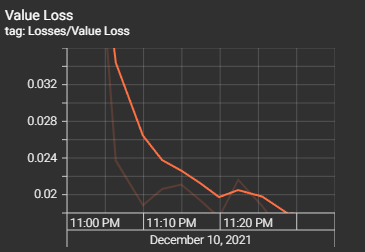
\includegraphics[width=0.30\textwidth]{images/v2/2/valueloss.png}}%
            \hfill % <-- Seperation
            \subcaptionbox{Entropy}{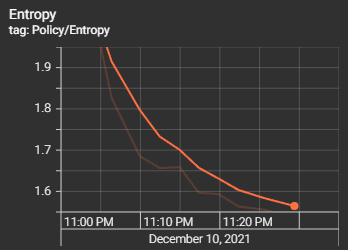
\includegraphics[width=0.30\textwidth]{images/v2/2/entroypy.png}}%
        \end{figure}
    \end{figure}
     
     \newpage
     
     \subsubsection{Versió 2.3}
    La versió 2.3 te dos processos d'aprenentatge, un amb el fitxer per defecte de configuració de mlagent i un fitxer de configuració costum.

    La versió 2.3 no és compatible amb les seves menors perquè el vector d'observacions de la xarxa neuronal generada és més gran, ja que percep una variable més, que l'estat atac, que no el de les xarxes de la versions 2.1 i 2.2 no el feien.
    
    La versió 2.3 arregla errors de la versió 2.2 com ara, evitar salts no necessaris, per autodefensa comença a fer múltiples salts, arregla el tema estètic referent al mode atac que es feia per un mal condicional, i finalment el important és la versió 2.3 que serà l'última, té com un dels camps a observar la variable global attackmode. D'aquesta manera se li dona més informació a l'algoritme d'aprenentatge, i és rellevant perquè és una variable, que segons el seu estat, es pot o no saltar, es pot o no entrar en mode atac.
    
    En l'última versió, vaig modificar el fitxer de configuració.yaml per defecte per multiplicar per deu la sessió d'entrenament, ja que veia que amb els 500000 passos per defecte que feia com a màxim no eren necessaris per aprendre correctament la política, també vaig augmentar el nombre de layers per neurona de dos a tres, i finalment vaig augmentar els hidden\_units de 128 a 256 per cada layer, a veure si d'aquesta manera el rendiment a trobar els patrons millorava. També vaig haver de fer sessions de treure el generador d'enemics (herois) i passar-los, perquè eviti aprendre que saltar per defensar-se sense cap enemic és cosa bona. I ja que puc generar rèpliques de l'escenari, també vaig fer modificacions a cada rèplica com ara, el període generació enemic, en què algunes hi hagi o no enemics i la variació de la velocitat pròpia del NPC.
    
        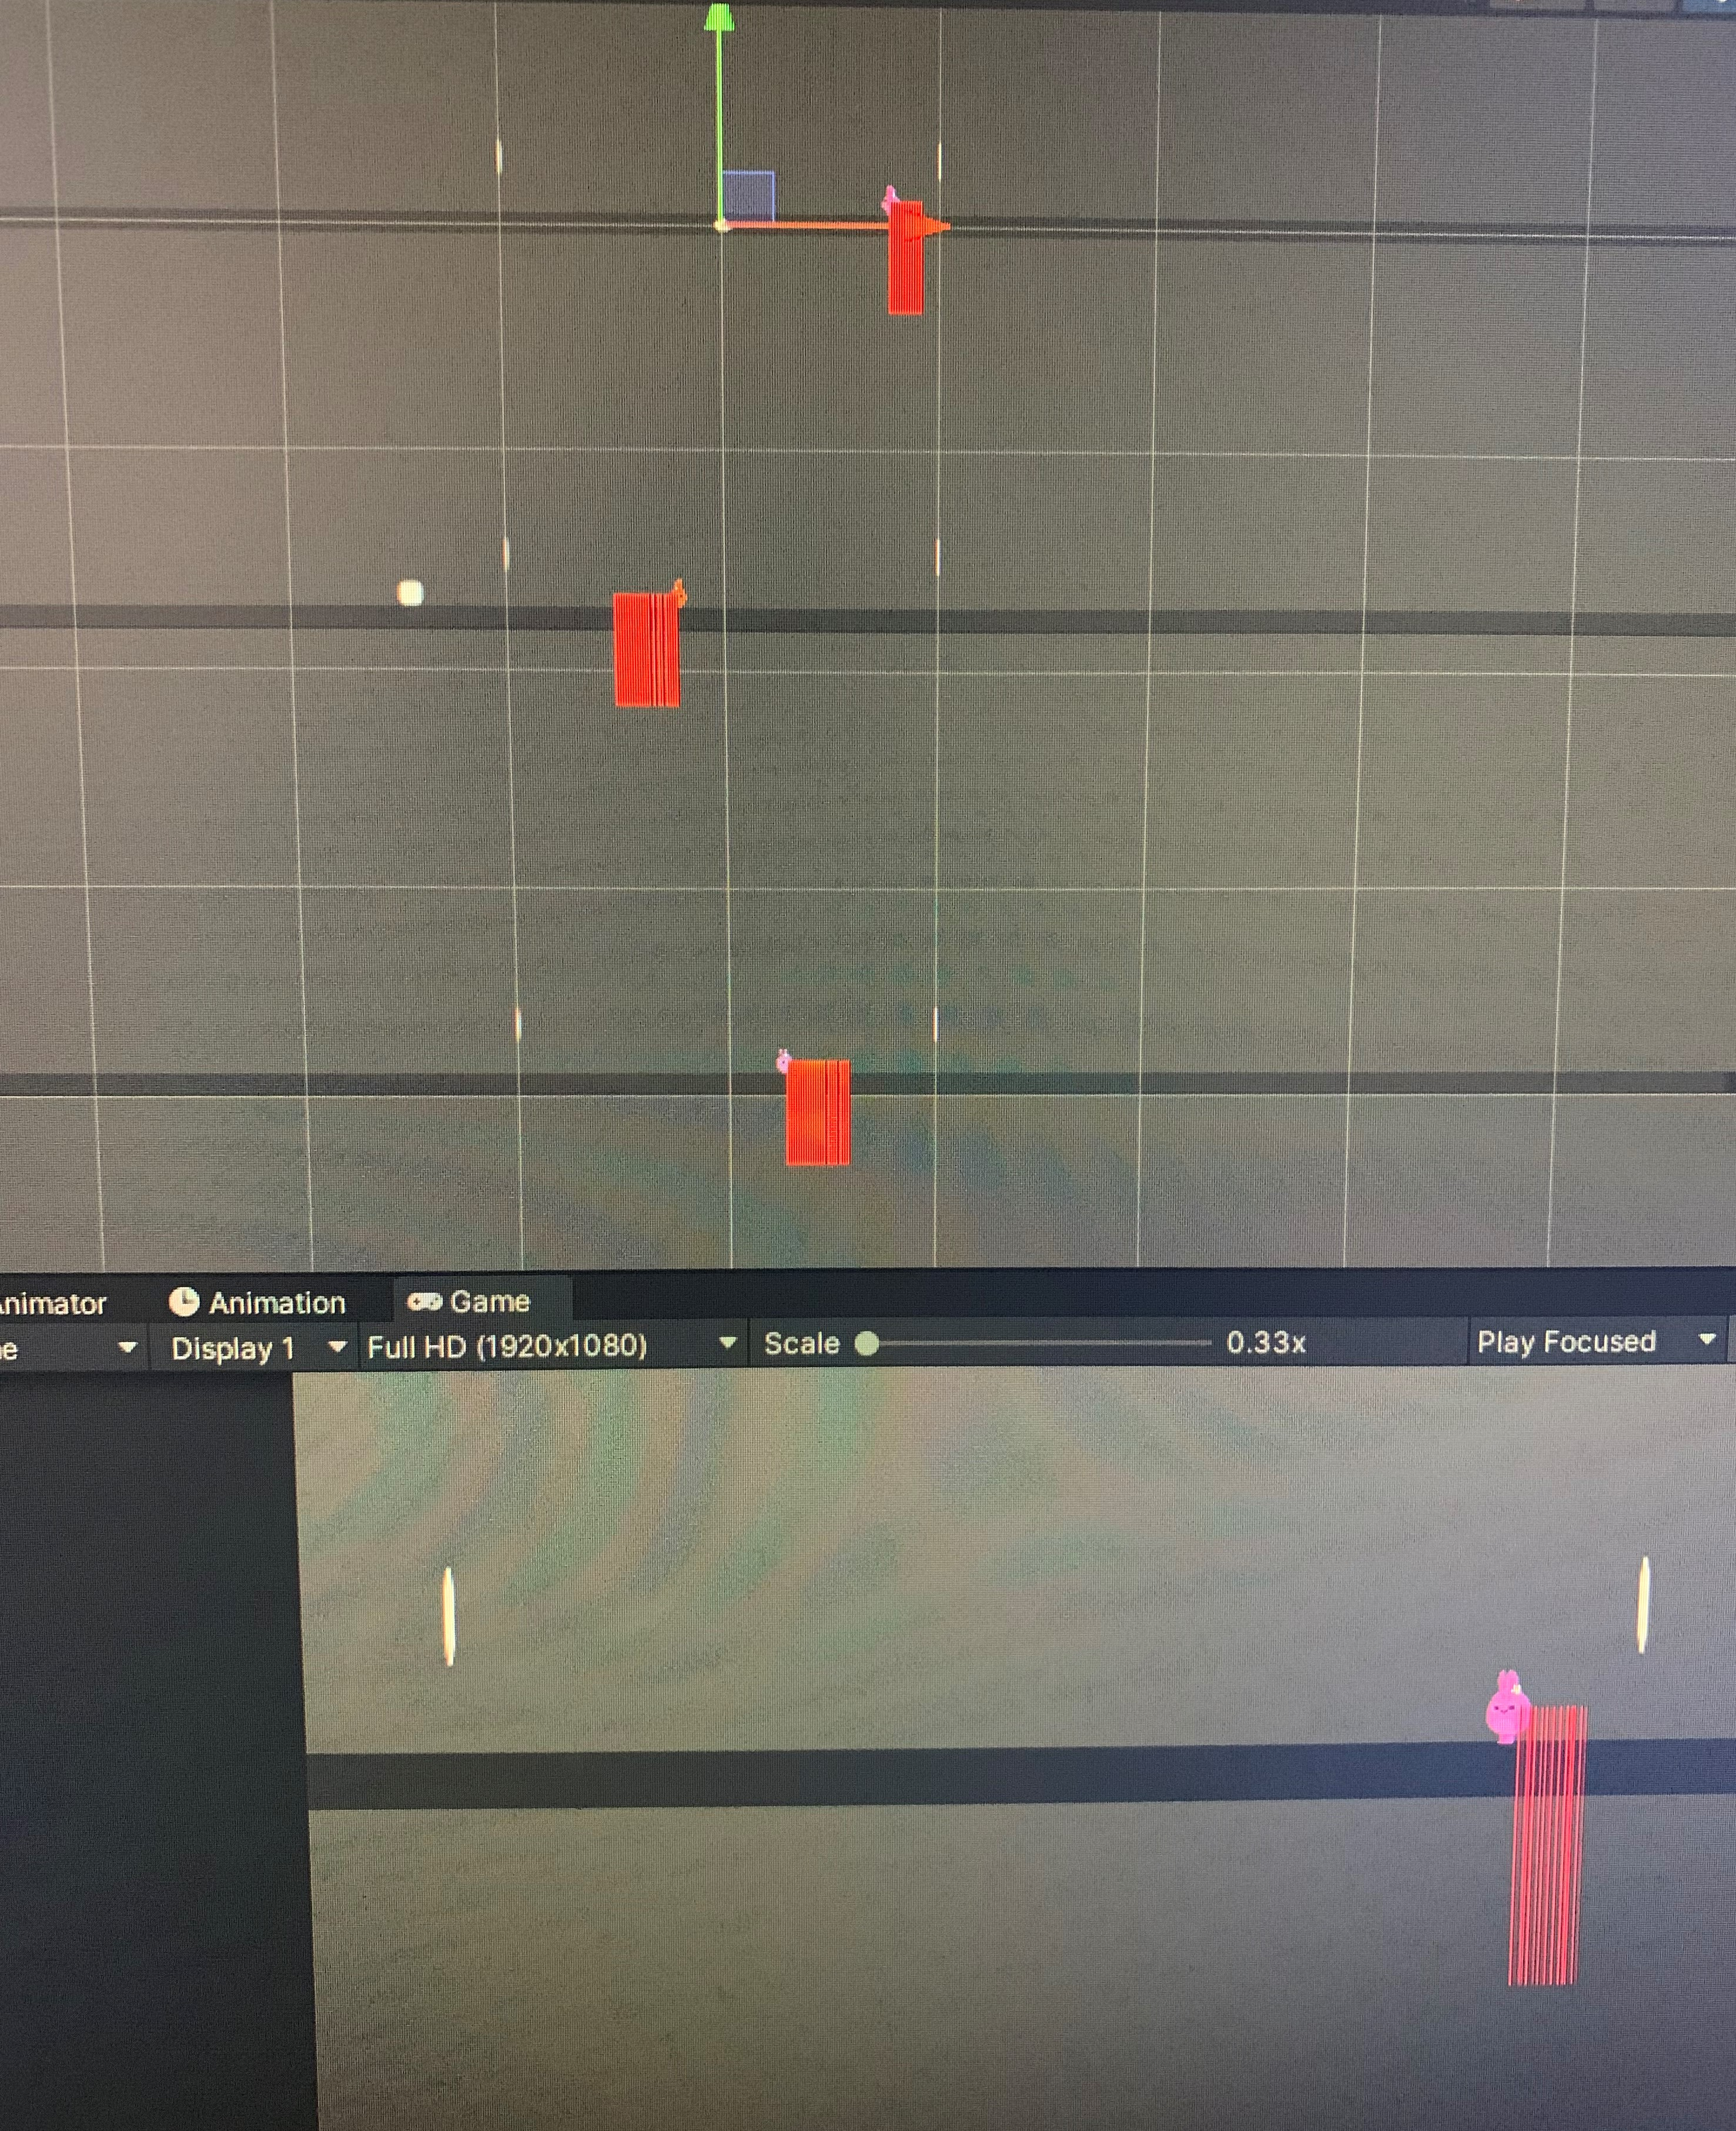
\includegraphics[width=1\textwidth]{images/v2/entrenamiento-multiple.jpg}
        
     \newpage
     
     En aquesta versió el canvi més important és que li dono informació al procés d'aprenentatge de l'estat de l'atac mode i el control correcte d'animacions de salts.
     
     \begin{lstlisting}
           public override void OnActionReceived(ActionBuffers actions)
    {
        int jump = actions.DiscreteActions[0];
        float xhorientation = actions.ContinuousActions[0];
        Vector2 v = rb.velocity;
        AddReward(-gain / 10000); // trying to finish the task quickly 

        // checking if the new orientantion action is good
        if (target && trainning)
        {
            Vector2 orientation = new Vector2(xhorientation, 0).normalized;
            float simil = Vector2.Dot(orientation, TargetDirectionNormalized());
	@@ -151,7 +151,7 @@ public override void OnActionReceived(ActionBuffers actions)

        }

        bool shouldJump = ShouldJump() && !attackMode; // SHOULD JUMP WHEN NOT IN MODE ATTACK TOO

        // try to learn not to jump when it is not in the ground
        bool unneededJump = jump == 1 && !shouldJump;
	@@ -171,11 +171,10 @@ public override void OnActionReceived(ActionBuffers actions)
            AddReward(gain / 10);
        }

        Vector2 movement = new Vector2(xhorientation * movementPower, jump == 1 && shouldJump ? jump * jumpPower : v.y); // CLAVE
        rb.velocity = movement;
        // run attack mode
        if (jump == 1 && shouldJump)
        {
            StartCoroutine(AttackModeCoroutine());
        }
    }
     \end{lstlisting}
     
     \begin{lstlisting}
             public override void CollectObservations(VectorSensor sensor)
    {
        if (!target) return;
        Vector2 currentPos = new Vector2(transform.position.x, 0);
        Vector2 targetPos = new Vector2(target.transform.position.x, 0);
        Vector2 toTarget = targetPos - currentPos;
        // 2 observations (horientation)
        sensor.AddObservation(toTarget.normalized);
        // 1 observation (distance)
        sensor.AddObservation(Vector2.Distance(targetPos, currentPos));
        // 2 observations for current target position
        sensor.AddObservation(targetPos);
        // 2 observations for movement velocity
        sensor.AddObservation(rb.velocity.normalized);
        // 1 observacion para mirar el modo ataque
        sensor.AddObservation(attackMode);
    }
     \end{lstlisting}
     
    Estadístiques llençades per Tensorboard de l'entrenament de la versió 2.3 amb 500000 steps.    
    \begin{figure}[H]
        \begin{figure}[H]
        \centering
            \subcaptionbox{Comulative reward}{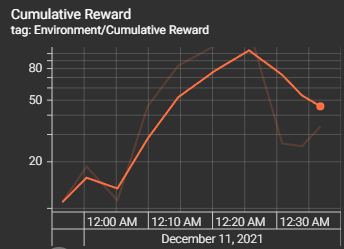
\includegraphics[width=0.30\textwidth]{images/v2/3/500000/cumulativereward.png}}%
            \hfill % <-- Seperation
            \subcaptionbox{Episodi length}{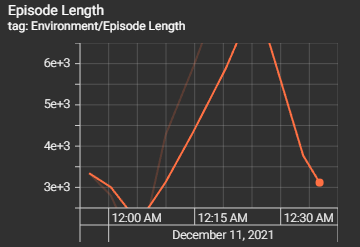
\includegraphics[width=0.30\textwidth]{images/v2/3/500000/episodilength.png}}%
            \hfill % <-- Seperation
            \subcaptionbox{Learning rate}{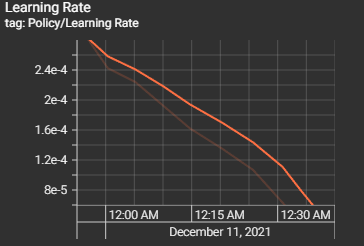
\includegraphics[width=0.30\textwidth]{images/v2/3/500000/learningrate.png}}%
            \hfill % <-- Seperation
             \subcaptionbox{Policity loss}{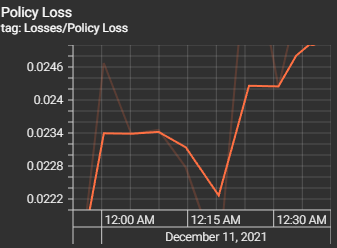
\includegraphics[width=0.30\textwidth]{images/v2/3/500000/policyloss.png}}%
            \hfill % <-- Seperation
            \subcaptionbox{Value Loss}{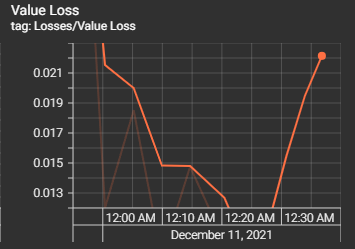
\includegraphics[width=0.30\textwidth]{images/v2/3/500000/valueloss.png}}%
            \hfill % <-- Seperation
            \subcaptionbox{Entropy}{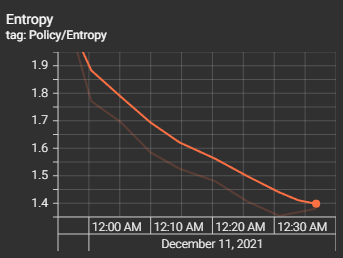
\includegraphics[width=0.30\textwidth]{images/v2/3/500000/entropy.png}}%
        \end{figure}
    \end{figure}
    
    \newpage
    
    Estadistiques llençades per Tensorboard de l'entrenament de la versió 2.3 amb el fitxer custom.
    
    \begin{figure}[H]
        \begin{figure}[H]
        \centering
            \subcaptionbox{Comulative reward}{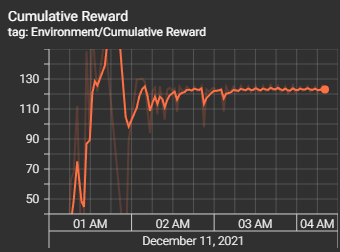
\includegraphics[width=0.30\textwidth]{images/v2/3/custom/cumulativereward.png}}%
            \hfill % <-- Seperation
            \subcaptionbox{Episodi length}{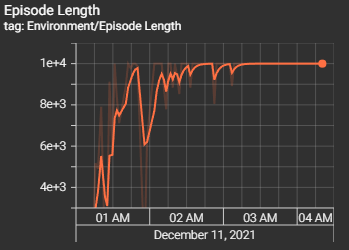
\includegraphics[width=0.30\textwidth]{images/v2/3/custom/episodilength.png}}%
            \hfill % <-- Seperation
            \subcaptionbox{Learning rate}{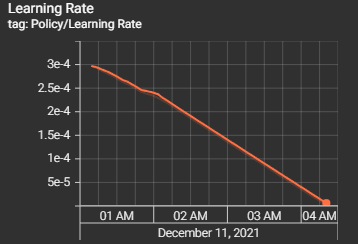
\includegraphics[width=0.30\textwidth]{images/v2/3/custom/learningrate.png}}%
            \hfill % <-- Seperation
             \subcaptionbox{Policity loss}{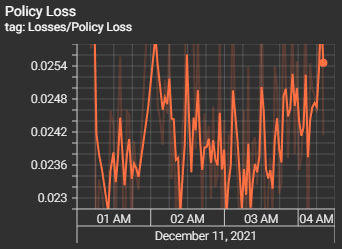
\includegraphics[width=0.30\textwidth]{images/v2/3/custom/policyloss.png}}%
            \hfill % <-- Seperation
            \subcaptionbox{Value Loss}{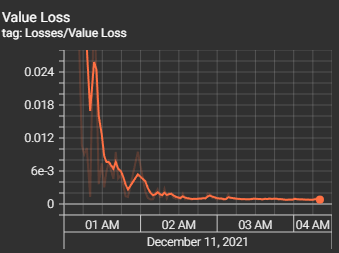
\includegraphics[width=0.30\textwidth]{images/v2/3/custom/valueloss.png}}%
            \hfill % <-- Seperation
            \subcaptionbox{Entropy}{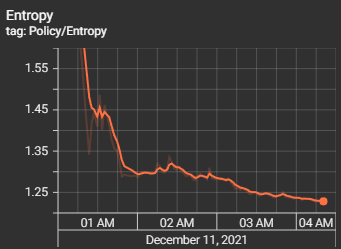
\includegraphics[width=0.30\textwidth]{images/v2/3/custom/entropy.png}}%
        \end{figure}
    \end{figure}
     
 
    \section{Conclusions i línies futures}
    
    Considero que el projecte ha estat un exit, s'han completat la majoria dels objectius, m'ha servit per tenir més clar en lo que es basa el Deep Learning i el Reinforcement Learning i finalment m'ha permes treballar una mica més amb l'eina principal que em prencipi utilitzaré per fer el TFG.
    
    Dic que s'han comples gairabe el cent per cent dels objectius perquè, una de les coses que tenia pensat d'implementar però per questions técniques referents a errors no vaig poder va ser que l'Agent quan detecti un enemic, canvi el seu target cap a ell. Tot i que l'Agent quan detecta un enemic es possa en mode atac i si l'enemic el toca a ell es mor, l'Agent continua amb el seu target de limits, però no fa una intensió real de dirigir-se al enemic proper.
    
    Aquesta ampliació de la modelització seria una de les possibles linies futures del projecte.
    
    Si estas interessat en l'implementació del projecte, et convido a visitar el meu \href{https://github.com/wilberquito/NPC}{repositori} en Github, a les altures d'haver entregat el projecte, el repositori hauria d'estar public.
    
    \section{Referències}
    
    \begin{thebibliography}{9}
    \bibitem{ml-agents}
    \emph{Unity ml-agents documentation \url{https://github.com/Unity-Technologies/ml-agents/tree/main/docs}}.
    
    \bibitem{plots}
    \emph{Understand machine learning plot results
    \url{https://medium.com/aureliantactics/understanding-ppo-plots-in-tensorboard-cbc3199b9ba2}}.
    
    \end{thebibliography}

\end{document}
